% figure-peak-argument-cases.tex — inline, no float wrapper.

\begin{center}
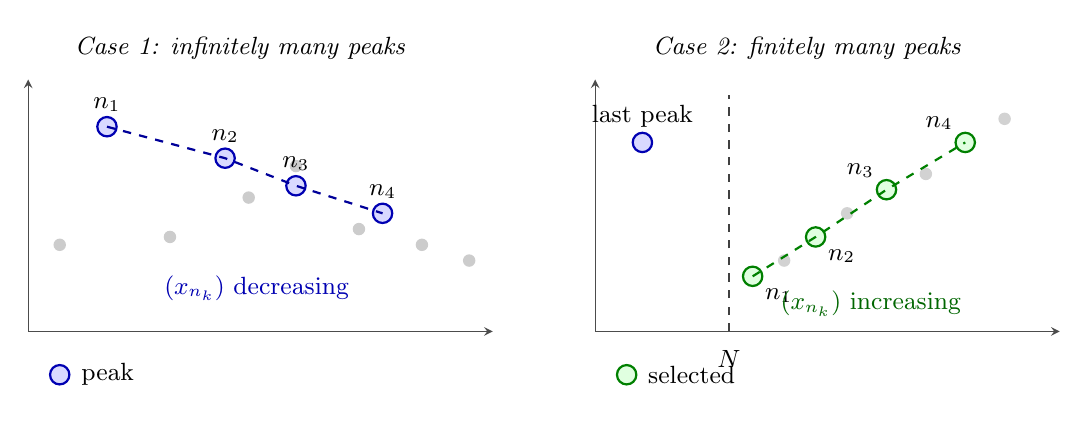
\begin{tikzpicture}[
  dot/.style={circle, fill, inner sep=0pt, minimum size=4.5pt},
  peak/.style={circle, draw=blue!70!black, fill=blue!15!white,
               inner sep=0pt, minimum size=7pt, thick},
  notpeak/.style={circle, draw=green!50!black, fill=green!12!white,
                  inner sep=0pt, minimum size=7pt, thick},
  lbl/.style={font=\small},
  arr/.style={->, >=stealth, thin, gray!60!black}
]
% LEFT: infinitely many peaks
\node[lbl, align=center] at (3.0, 3.6) {\textit{Case 1: infinitely many peaks}};
\draw[arr] (0.3, 0) -- (6.2, 0);
\draw[arr] (0.3, 0) -- (0.3, 3.2);
\foreach \x/\y in {0.7/1.1, 1.3/2.6, 2.1/1.2, 3.1/1.7,
                   3.7/2.1, 4.5/1.3, 5.3/1.1, 5.9/0.9}
  \node[dot, fill=gray!40!white] at (\x, \y) {};
\node[peak] (p1) at (1.3, 2.6) {};
\node[peak] (p2) at (2.8, 2.2) {};
\node[peak] (p3) at (3.7, 1.85) {};
\node[peak] (p4) at (4.8, 1.5) {};
\node[lbl, above=2pt] at (1.3, 2.6) {$n_1$};
\node[lbl, above=2pt] at (2.8, 2.2) {$n_2$};
\node[lbl, above=2pt] at (3.7, 1.85) {$n_3$};
\node[lbl, above=2pt] at (4.8, 1.5) {$n_4$};
\draw[dashed, blue!60!black, thick]
  (1.3, 2.6) -- (2.8, 2.2) -- (3.7, 1.85) -- (4.8, 1.5);
\node[lbl, text=blue!70!black] at (3.2, 0.55) {$(x_{n_k})$ decreasing};
\node[peak] at (0.7, -0.55) {};
\node[lbl, right] at (0.85, -0.55) {peak};
% RIGHT: finitely many peaks
\begin{scope}[xshift=7.2cm]
\node[lbl, align=center] at (3.0, 3.6) {\textit{Case 2: finitely many peaks}};
\draw[arr] (0.3, 0) -- (6.2, 0);
\draw[arr] (0.3, 0) -- (0.3, 3.2);
\node[peak] at (0.9, 2.4) {};
\node[lbl, above=2pt] at (0.9, 2.4) {last peak};
\draw[dashed, gray!50!black] (2.0, 0) -- (2.0, 3.0);
\node[lbl, below] at (2.0, -0.12) {$N$};
\node[notpeak] (q1) at (2.3, 0.7) {};
\node[notpeak] (q2) at (3.1, 1.2) {};
\node[notpeak] (q3) at (4.0, 1.8) {};
\node[notpeak] (q4) at (5.0, 2.4) {};
\node[lbl, below right=1pt] at (2.3, 0.7) {$n_1$};
\node[lbl, below right=1pt] at (3.1, 1.2) {$n_2$};
\node[lbl, above left=1pt] at (4.0, 1.8) {$n_3$};
\node[lbl, above left=1pt] at (5.0, 2.4) {$n_4$};
\foreach \x/\y in {2.7/0.9, 3.5/1.5, 4.5/2.0, 5.5/2.7}
  \node[dot, fill=gray!35!white] at (\x, \y) {};
\draw[dashed, green!50!black, thick]
  (2.3, 0.7) -- (3.1, 1.2) -- (4.0, 1.8) -- (5.0, 2.4);
\node[lbl, text=green!40!black] at (3.8, 0.35) {$(x_{n_k})$ increasing};
\node[notpeak] at (0.7, -0.55) {};
\node[lbl, right] at (0.85, -0.55) {selected};
\end{scope}
\end{tikzpicture}
\end{center}
\captionof{figure}{%
  The two cases of the Monotone Subsequence Theorem
  (\cref{thm:monotone-subsequence}).
  \textit{Left:} Infinitely many peaks (blue) yield a decreasing
  subsequence (dashed blue).
  \textit{Right:} After the last peak, every $n \geq N$ is a non-peak,
  so a later term always exceeds the current one; this fuels the inductive
  construction of an increasing subsequence (dashed green).%
}
\label{fig:peak-argument-cases}
\medskip
